\documentclass[11pt, letterpaper]{article}
\usepackage[utf8]{inputenc}
\usepackage{geometry}
\usepackage{fancyhdr}
\usepackage{amsmath, amssymb}
\usepackage{xcolor}
\usepackage{listings}
\usepackage{enumitem}
\usepackage{hyperref}
\usepackage{graphicx}
\usepackage{booktabs}
\newcommand{\E}{\mathbb{E}}
\newcommand{\Var}{\mathrm{Var}}

% Make parindent 0
\setlength{\parindent}{0pt}
\setlist{itemsep=0.5em}
\setlength{\parskip}{0.5em}

\geometry{margin=1in}
\pagestyle{fancy}
\fancyhf{}
\lhead{\textbf{Solutions}}
\rhead{\textbf{Data Analysis and Regression, Homework 2}}
\cfoot{\thepage}

\definecolor{codegreen}{rgb}{0,0.6,0}
\definecolor{codegray}{rgb}{0.5,0.5,0.5}
\definecolor{codepurple}{rgb}{0.58,0,0.82}
\definecolor{backcolour}{rgb}{0.95,0.95,0.92}

\lstdefinestyle{mystyle}{
    backgroundcolor=\color{backcolour},   
    commentstyle=\color{codegreen},
    keywordstyle=\color{magenta},
    numberstyle=\tiny\color{codegray},
    stringstyle=\color{codepurple},
    basicstyle=\ttfamily\footnotesize,
    breakatwhitespace=false,         
    breaklines=true,                 
    captionpos=b,                    
    keepspaces=true,                 
    numbers=left,                    
    numbersep=5pt,                  
    showspaces=false,                
    showstringspaces=false,
    showtabs=false,                  
    tabsize=2
}
\lstset{style=mystyle}

\newcommand{\problem}[1]{\section*{Problem #1}}
\newcommand{\subproblem}[1]{\subsection*{Problem #1}}
\newcommand{\answer}{\textbf{\textit{\textcolor{red}{Answer:}}}\\}

\begin{document}

\section*{Instructions}
\begin{itemize}
    \item Homework 2 was due Wednesday, July 29th at 18:00 Chicago Time.
    \item All numbers and figures come from \texttt{homework\_2\_solution.ipynb}, run from top to bottom.
\end{itemize}
\hrule
\vspace{0.5cm}

\pagebreak

\problem{1: Hands-On OLS}

\subproblem{1.1: Setup}

Set your random seed using \texttt{np.random.seed(1)}. Generate $n=30$ observations where:
\begin{itemize}
    \item The predictor $X$ is drawn from a standard normal distribution, $X \sim N(0, 1)$.
    \item The error term $\epsilon$ is drawn from a normal distribution with mean 0 and standard deviation 1, $\epsilon \sim N(0, 1)$.
    \item The response variable is generated by the true relationship: $Y = 5 + 2X + \epsilon$.
\end{itemize}

Display a scatter plot of the generated data points $(X_i, Y_i)$.

\answer
\begin{center}
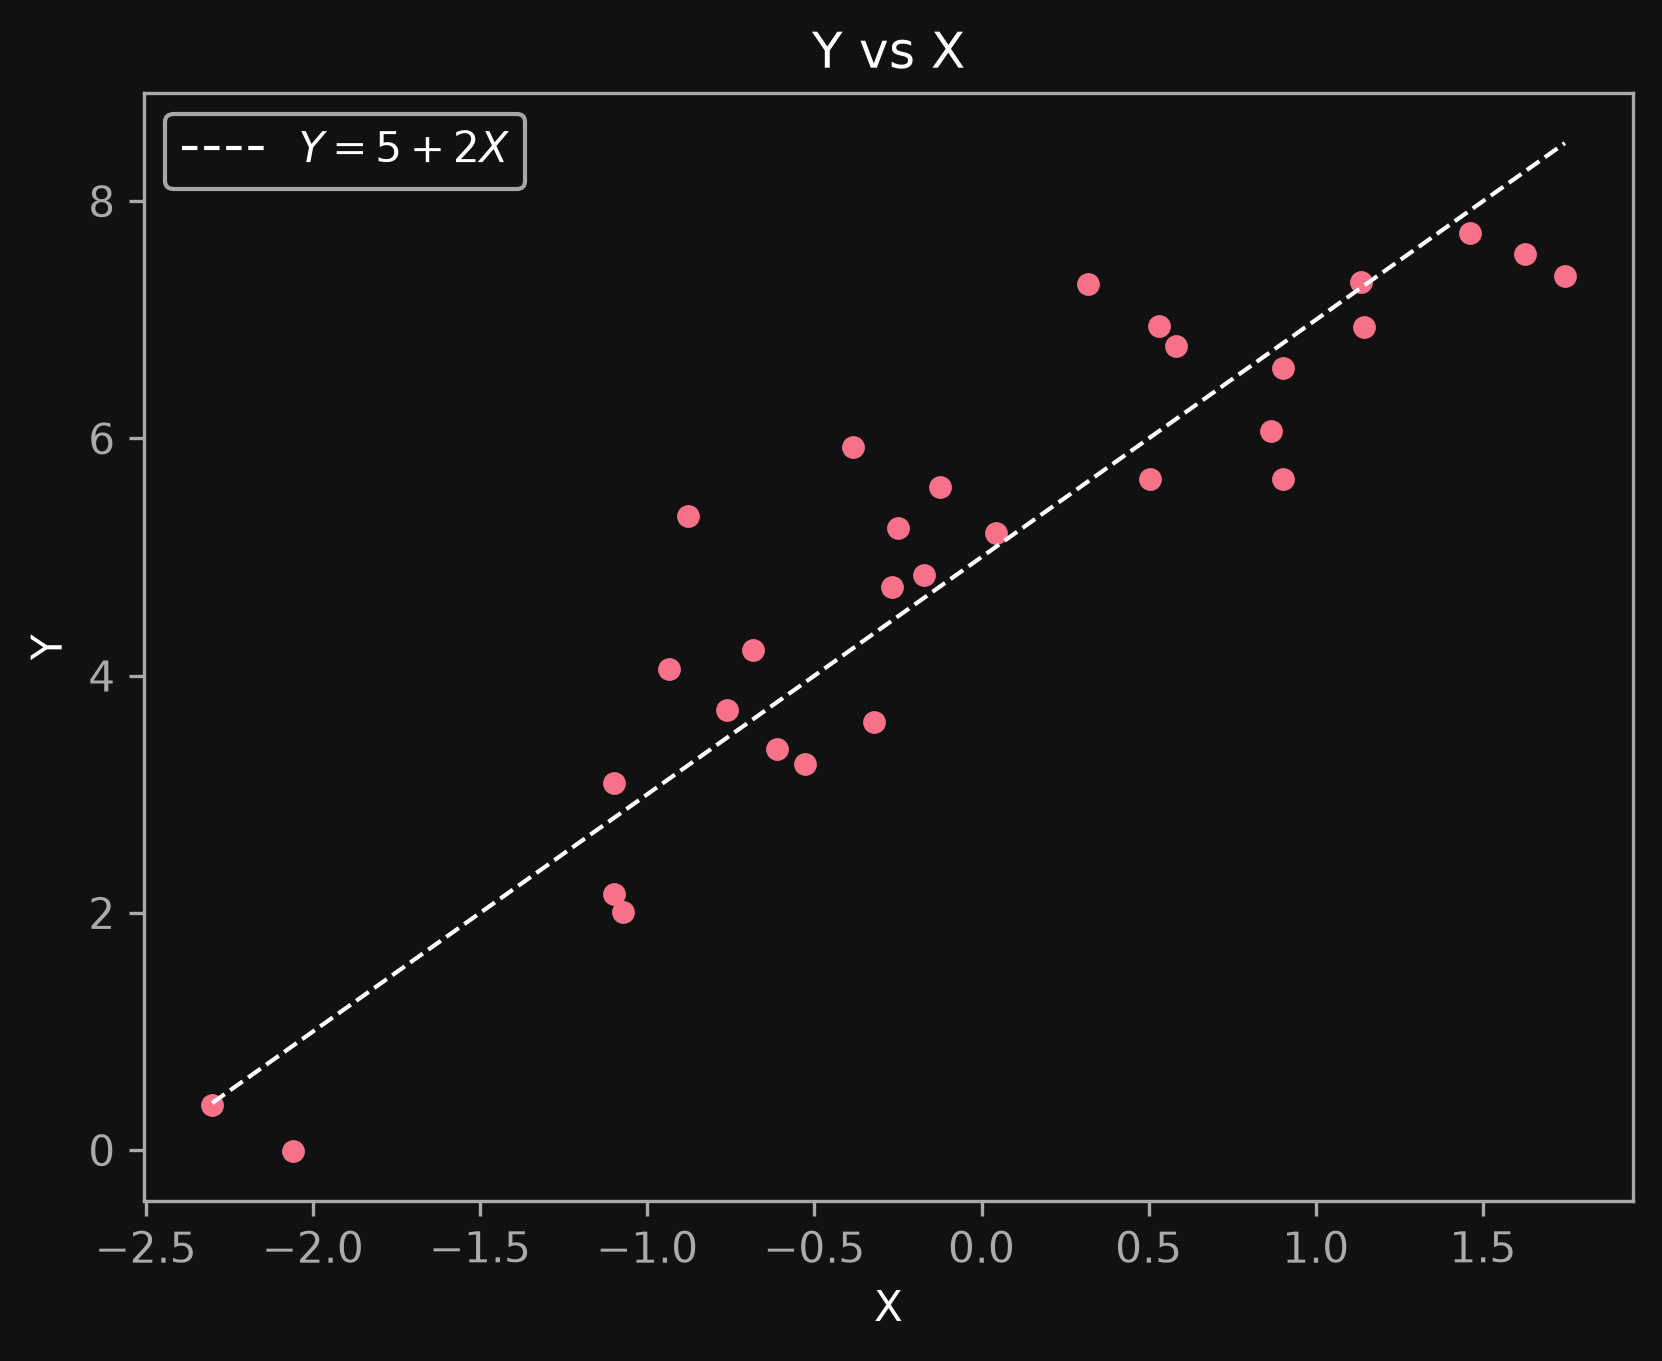
\includegraphics[width=0.58\textwidth]{./figures/problem1_scatter.png}
\end{center}


\subproblem{1.2: A First Fit}

Using the data generated above, fit an OLS model. You should report:
\begin{enumerate}
    \item $\hat{\beta}_0$ and $\hat{\beta}_1$ estimates.
    \item Your confidence intervals and p-values for both coefficients.
    \item The $R^2$ value of your fit.
\end{enumerate}

\answer
$R^2 = 0.840$ (adjusted $0.834$).

\begin{center}
\begin{tabular}{lcccccc}
\toprule
               & \textbf{coef} & \textbf{std err} & \textbf{t} & \textbf{P$> |$t$|$} & \textbf{[0.025} & \textbf{0.975]}  \\
\midrule
\textbf{const} &       5.0677  &        0.155     &    32.787  &         0.000        &        4.751    &        5.384     \\
\textbf{X}     &       1.8516  &        0.153     &    12.110  &         0.000        &        1.538    &        2.165     \\
\bottomrule
\end{tabular}
\end{center}


\subproblem{1.3: Interpretation}

How do your estimated coefficients and confidence intervals compare to the true parameters?

\answer
Close. $\hat{\beta}_0 = 5.0677$ against a true $5$, and $\hat{\beta}_1 = 1.8516$ against a true $2$,
and both intervals cover the truth: $5 \in [4.751,\, 5.384]$ and $2 \in [1.538,\, 2.165]$. Both
p-values round to $0$, so both coefficients are significant. With $n = 30$ the intervals are still
about $\pm 0.31$ wide, so this is not a precise fit -- only a correct one.


\subproblem{1.4: An Influential Point}

Now, modify your dataset by overriding the last observation to be the point $(X_{30}, Y_{30}) = (4, -5)$.
Refit your OLS model to this modified dataset, and report:
\begin{enumerate}
    \item $\hat{\beta}_0$ and $\hat{\beta}_1$ estimates.
    \item Your confidence intervals and p-values for both coefficients.
    \item The $R^2$ value of your fit.
\end{enumerate}

\answer
$R^2 = 0.027$ (adjusted $-0.008$).

\begin{center}
\begin{tabular}{lcccccc}
\toprule
               & \textbf{coef} & \textbf{std err} & \textbf{t} & \textbf{P$> |$t$|$} & \textbf{[0.025} & \textbf{0.975]}  \\
\midrule
\textbf{const} &       4.5388  &        0.500     &     9.082  &         0.000        &        3.515    &        5.563     \\
\textbf{X}     &       0.3533  &        0.402     &     0.879  &         0.387        &       -0.470    &        1.177     \\
\bottomrule
\end{tabular}
\end{center}

\subproblem{1.5: Interpretation}

How do your estimated coefficients and confidence intervals compare to the true parameters?

\answer
One point out of thirty destroys the fit. The slope falls from $1.8516$ to $0.3533$, its interval
widens from $\pm 0.31$ to $\pm 0.82$ and now contains zero, the p-value rises from $0.000$ to
$0.387$, and $R^2$ falls from $0.840$ to $0.027$.

The true slope of $2$ is now outside the interval, so the model has gone from correct and
significant to wrong and insignificant.


\subproblem{1.6: Cook's Distance}

Calculate Cook's distance for all observations in the modified dataset from Problem 1.4.
Plot the Cook's distance values, and highlight the 30th observation.

\answer
Cook's distance for observation 30 is $7.4530$. The largest of the other twenty-nine is $0.1676$, so
it is more than forty times the next worst point.

\begin{center}
\begin{minipage}{0.48\textwidth}
    \centering
    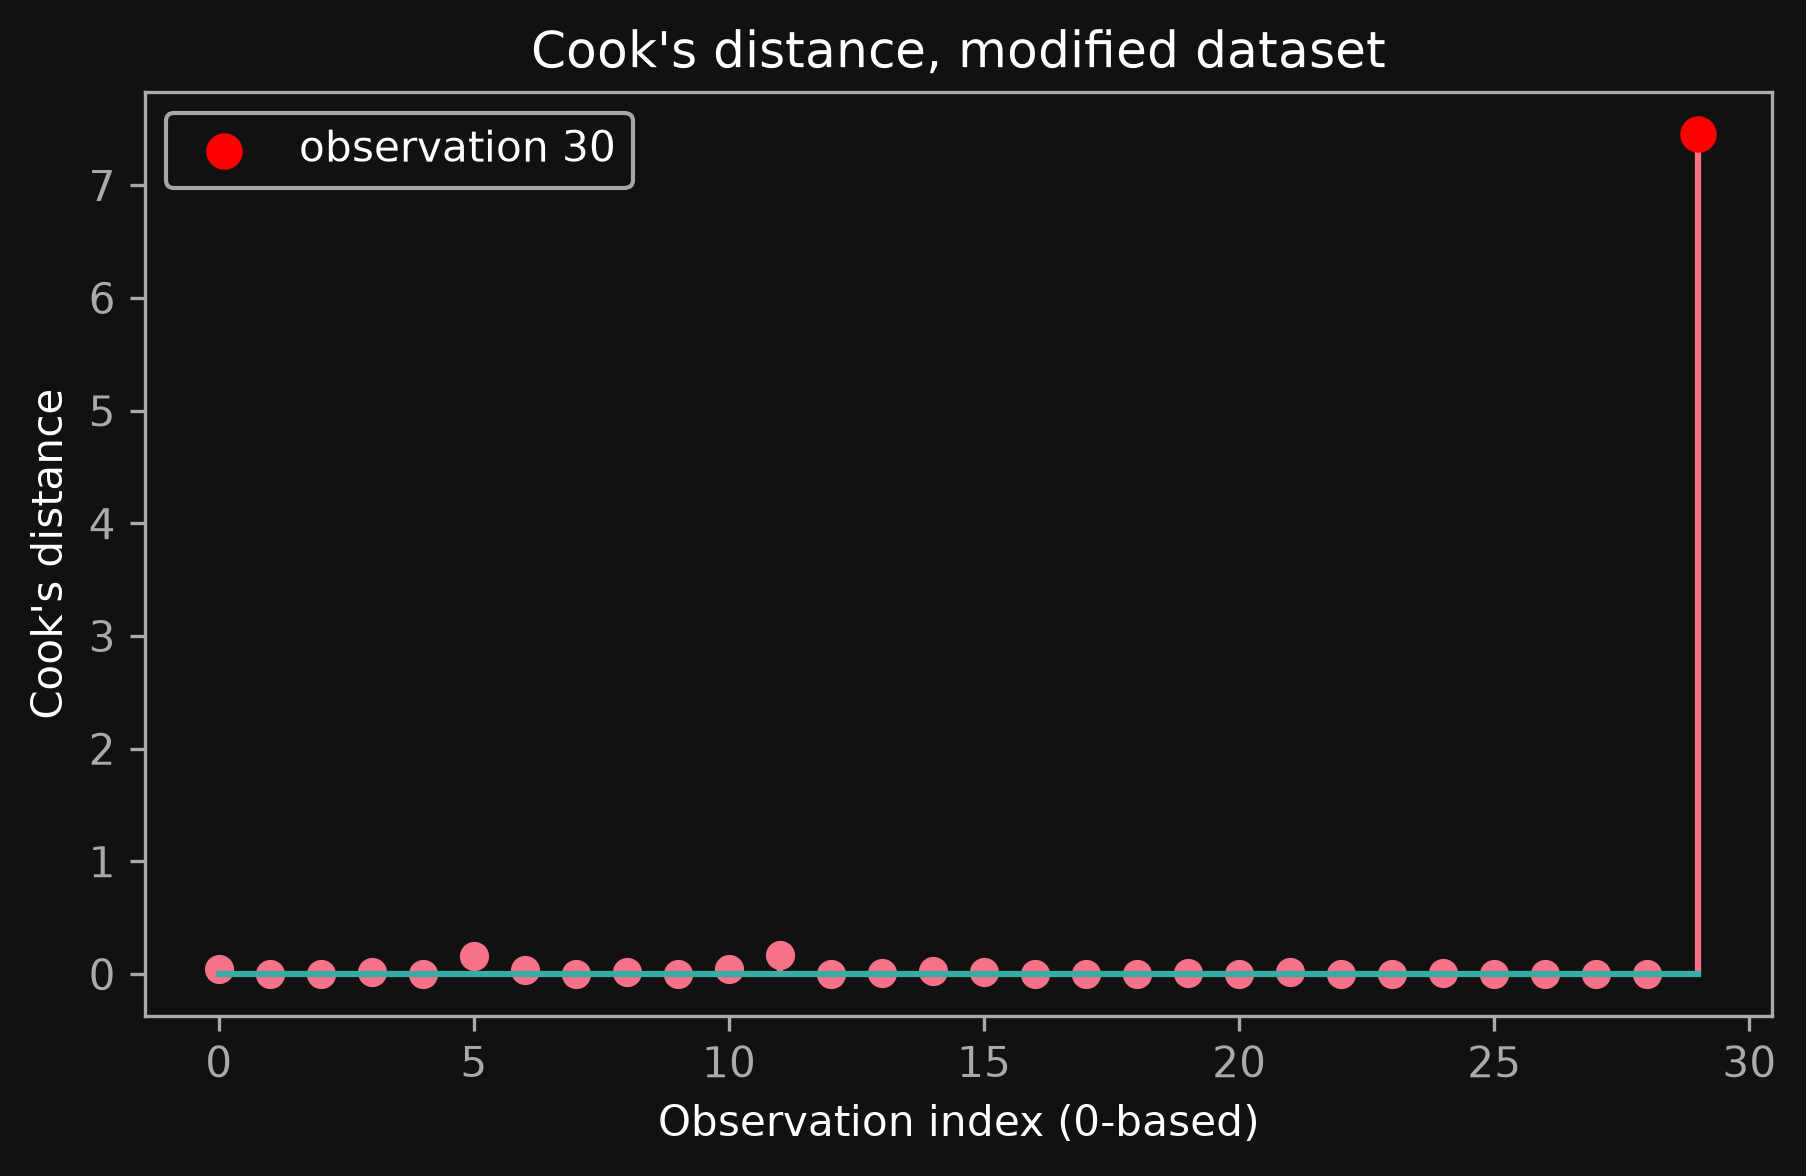
\includegraphics[width=\textwidth]{./figures/problem1_cooks_distance.png}
\end{minipage}
\hfill
\begin{minipage}{0.48\textwidth}
    \centering
    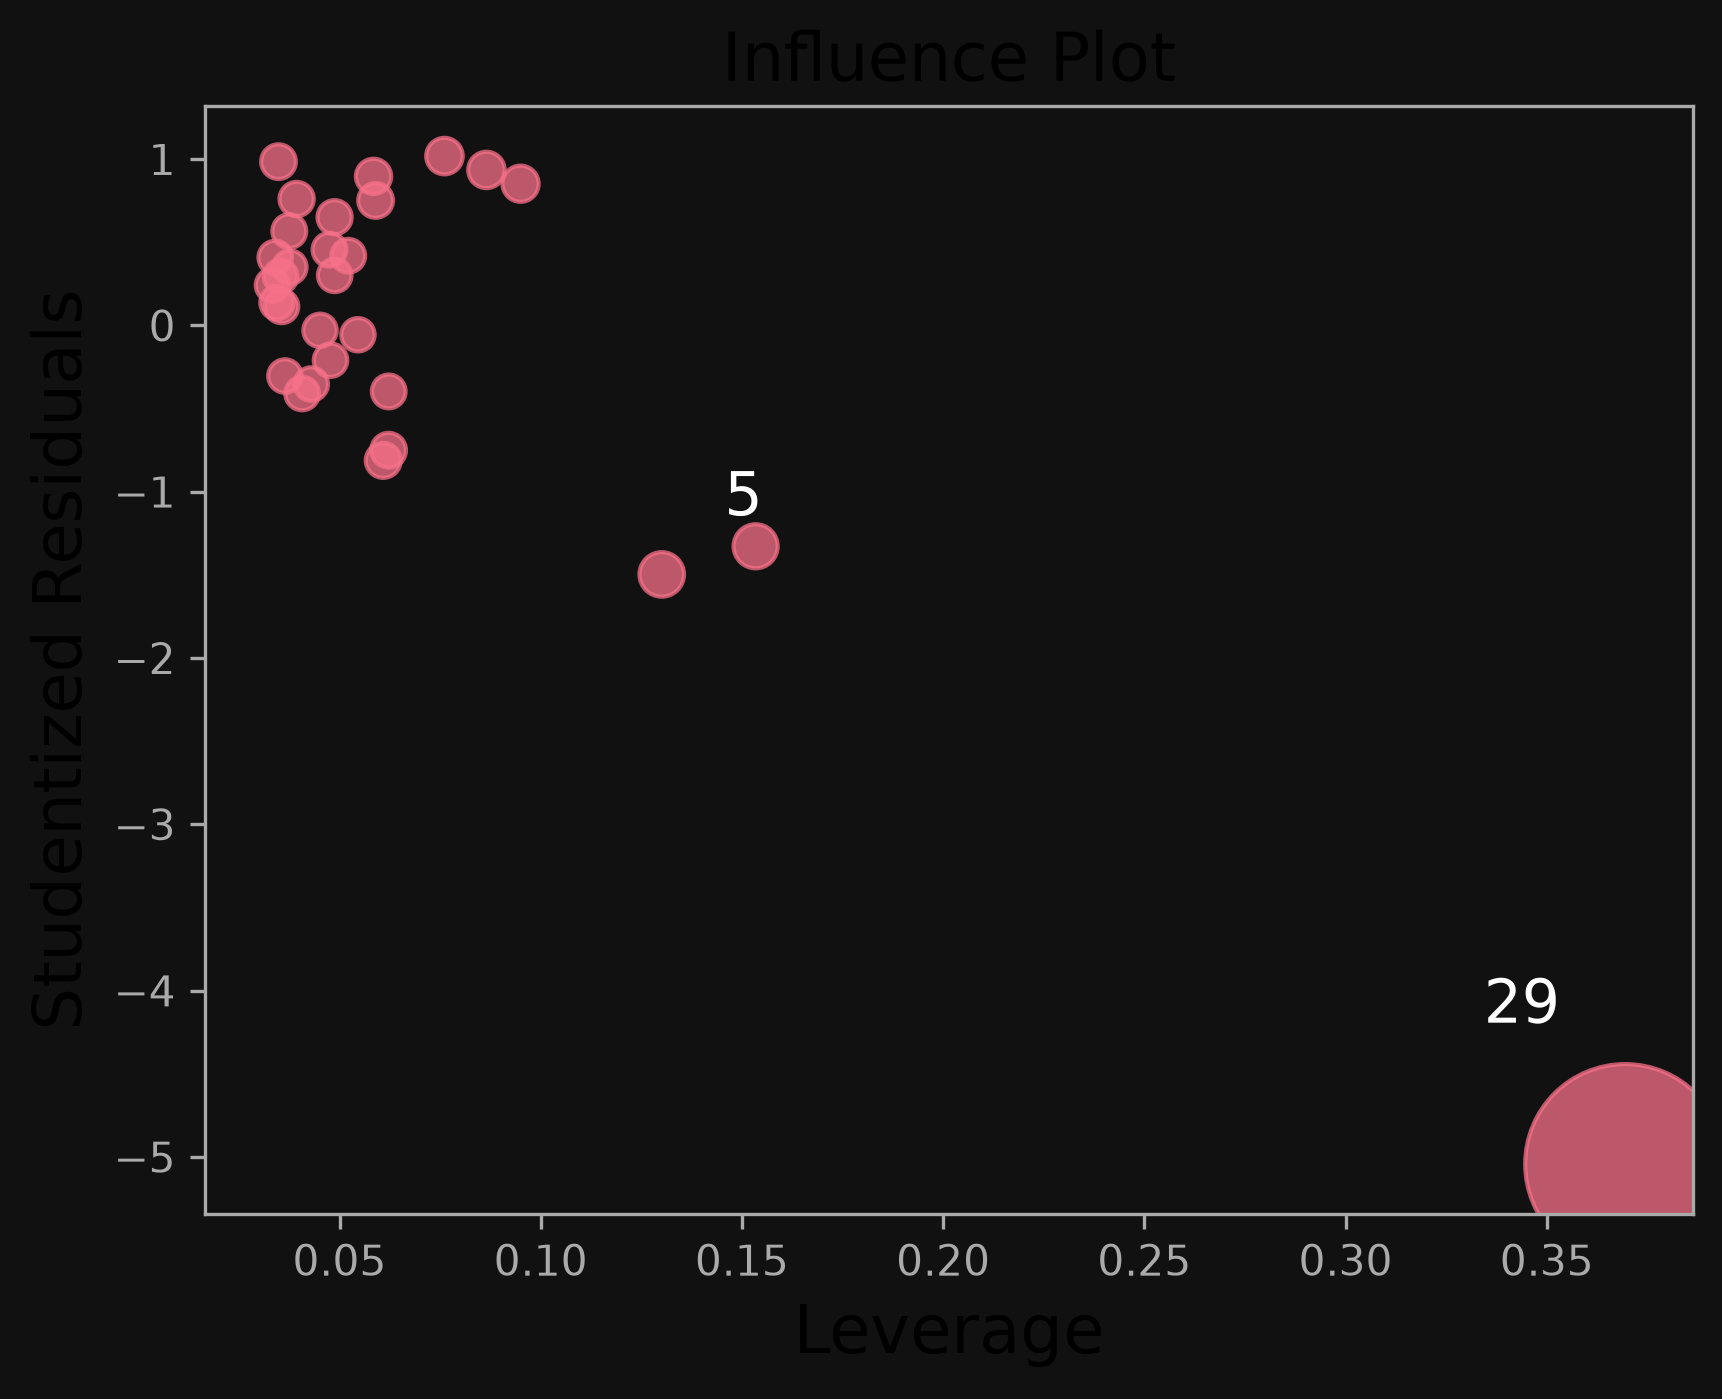
\includegraphics[width=\textwidth]{./figures/problem1_influence_plot.png}
\end{minipage}
\end{center}


\subproblem{1.7: What if?}

Suppose instead that the influential point you just added was $(X_{30}, Y_{30}) = (0, -5)$.

What would you expect the \textit{leverage} of this point to be relative to the $(4, -5)$ point you added before?

\answer
Much lower. For a fit with an intercept,
$$
h_{ii} = \frac{1}{n} + \frac{(x_i - \bar{x})^2}{\sum_{j} (x_j - \bar{x})^2},
$$
so leverage is driven by distance from $\bar{x}$, and $\bar{x} \approx 0$ here. Moving the point from
$x = 4$ to $x = 0$ drops the second term to almost nothing and leaves $h_{30}$ at the floor of
$1/n = 0.0333$.

\begin{center}
\begin{tabular}{lrrr}
\toprule
point & $h_{30}$ & Cook's $D_{30}$ & $\hat{\beta}_1$ \\
\midrule
$(4, -5)$ & 0.3695 & 7.4530 & 0.3533 \\
$(0, -5)$ & 0.0335 & 0.4059 & 1.8077 \\
\bottomrule
\end{tabular}
\end{center}

The point is just as far off the line in both cases, but without leverage it cannot pull the slope:
$\hat{\beta}_1$ stays at $1.8077$ against the $1.8516$ of the clean fit.



\problem{2: Central Limit Theorem}

We found in Class 2, that if $\epsilon_i \sim \mathcal{N}(0, \sigma^2)$,
then as $n \to \infty$, then $\beta_{\text{OLS}} \to \mathcal{N}(\beta_{\text{OLS}}, \sigma_{\text{OLS}}^2)$, where $\sigma_{\text{OLS}}^2 = \sigma^2 / \sum_{i=1}^n (x_i - \bar{x})^2$.

The goal of this problem is for you to empirically verify that this 
results holds \textit{even if} $\epsilon_i$ are not normally distributed.

\subproblem{2.1: Setup}

First, define the true model as:

$$
y = 2x
$$

Where $x$ is sampled from the uniform distribution $x \sim \text{Uniform}(0, 1)$.
Note that we are not including an intercept, nor any noise.

Second, define the noise $\epsilon_i$ to be sampled from 2 different distributions:
\begin{itemize}
    \item A Bernoulli distribution with $p=0.5$, and values $\{-1, 1\}$ (the Rademacher distribution).
    \item A uniform distribution with $\epsilon_i \sim \text{Uniform}(-1, 1)$.
\end{itemize}

For $n=500$, please display histograms of the 2 noise distributions you defined above.

\answer
\begin{center}
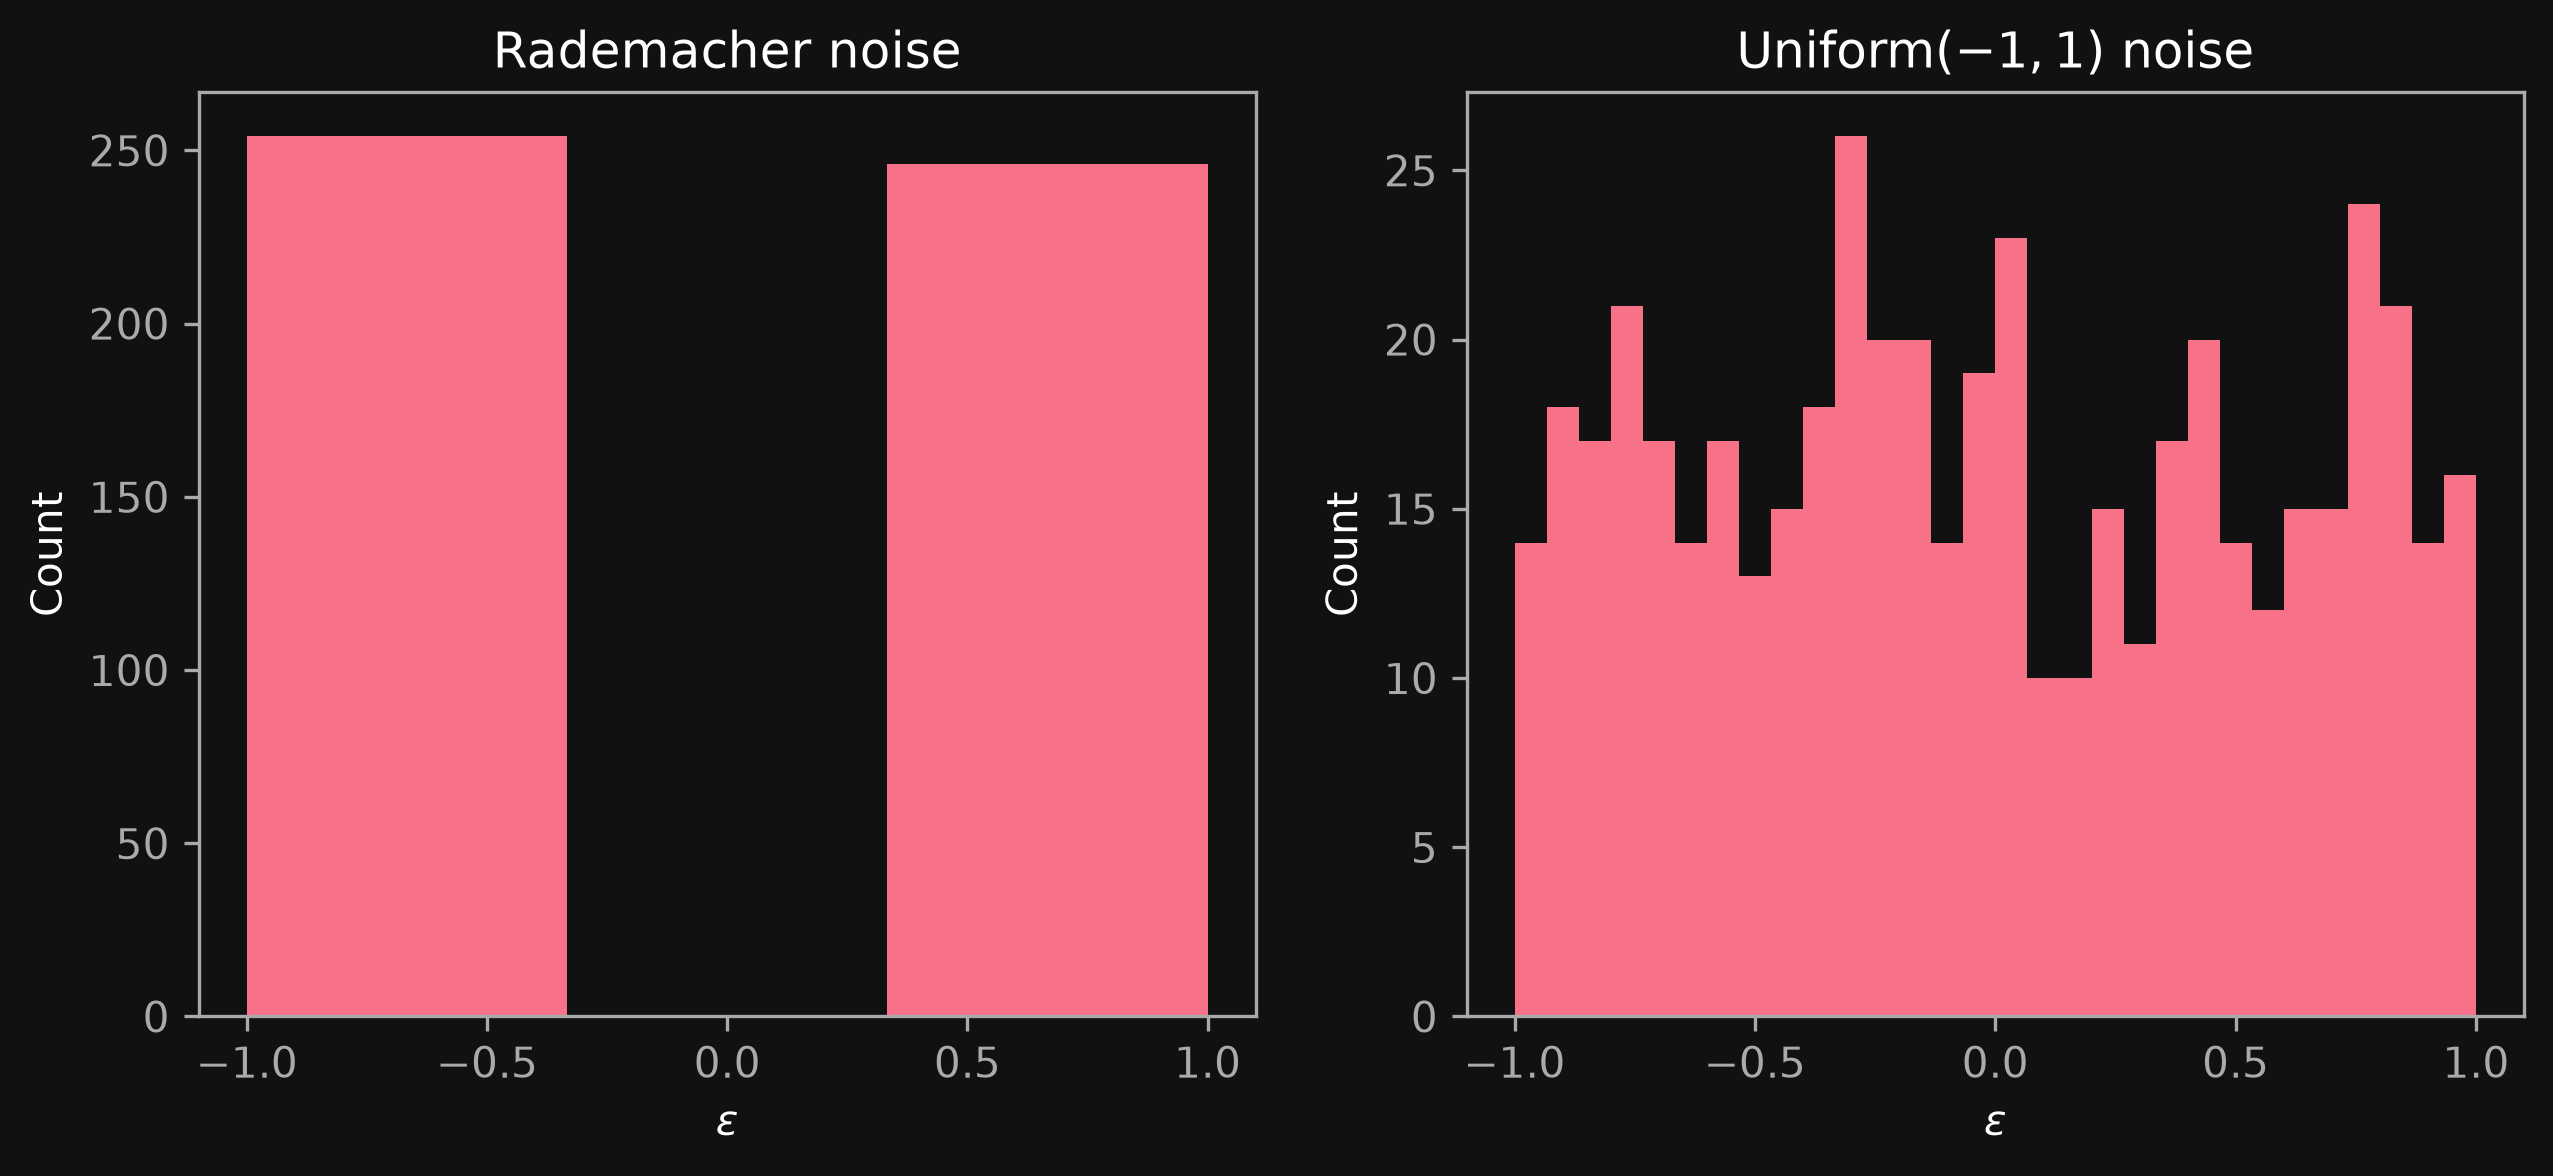
\includegraphics[width=0.95\textwidth]{./figures/problem2_error_histograms.png}
\end{center}


\subproblem{2.2: Empirical Verification}

\textbf{Note:} You should not re-sample your $x$ values, only the $\epsilon_i$ values.
That is, you should have a fixed set of $x$ values for this entire problem.

For $n \in {10, 100, 1000}$, and for each noise distribution defined above, do the following:
\begin{enumerate}
    \item Sample $n$ values of $\epsilon_i$ from the noise distribution.
    \item Generate the target values as $y_i = 2x_i + \epsilon_i$.
    \item Fit an OLS regression to the data $(x_i, y_i)$, and obtain the estimate $\hat{\beta}_{\text{OLS}}$.
    \item Repeat (1)-(3) 1,000 times, and save all of the $\hat{\beta}_{\text{OLS}}$ estimates.
\end{enumerate}
You should now have 6 sets of 1,000 $\hat{\beta}_{\text{OLS}}$ estimates (2 noise distributions $\times$ 3 values of $n$).

Include your simulation code below:

\answer
\begin{lstlisting}[language=Python]
res_beta = {}
x = np.random.rand(1000)  # fixed for the whole problem; only the noise is resampled
for n in [10, 100, 1000]:
    x_n = x[:n]
    draws = {"beta1": [], "beta2": []}
    for _ in range(1000):
        eps1 = 2 * np.random.binomial(1, 0.5, n) - 1
        eps2 = 2 * np.random.rand(n) - 1
        draws["beta1"].append(sm.OLS(2 * x_n + eps1, x_n).fit().params[-1])
        draws["beta2"].append(sm.OLS(2 * x_n + eps2, x_n).fit().params[-1])
    res_beta[n] = pd.DataFrame(draws)
\end{lstlisting}


\subproblem{2.3: Visualization}

For each of the 6 sets of $\hat{\beta}_{\text{OLS}}$ estimates obtained above, plot a histogram of the estimates.
Additionally, conduct a Shapiro-Wilk test for normality on each set of estimates,
report your p-values, and briefly discuss your results.

\answer
\begin{center}
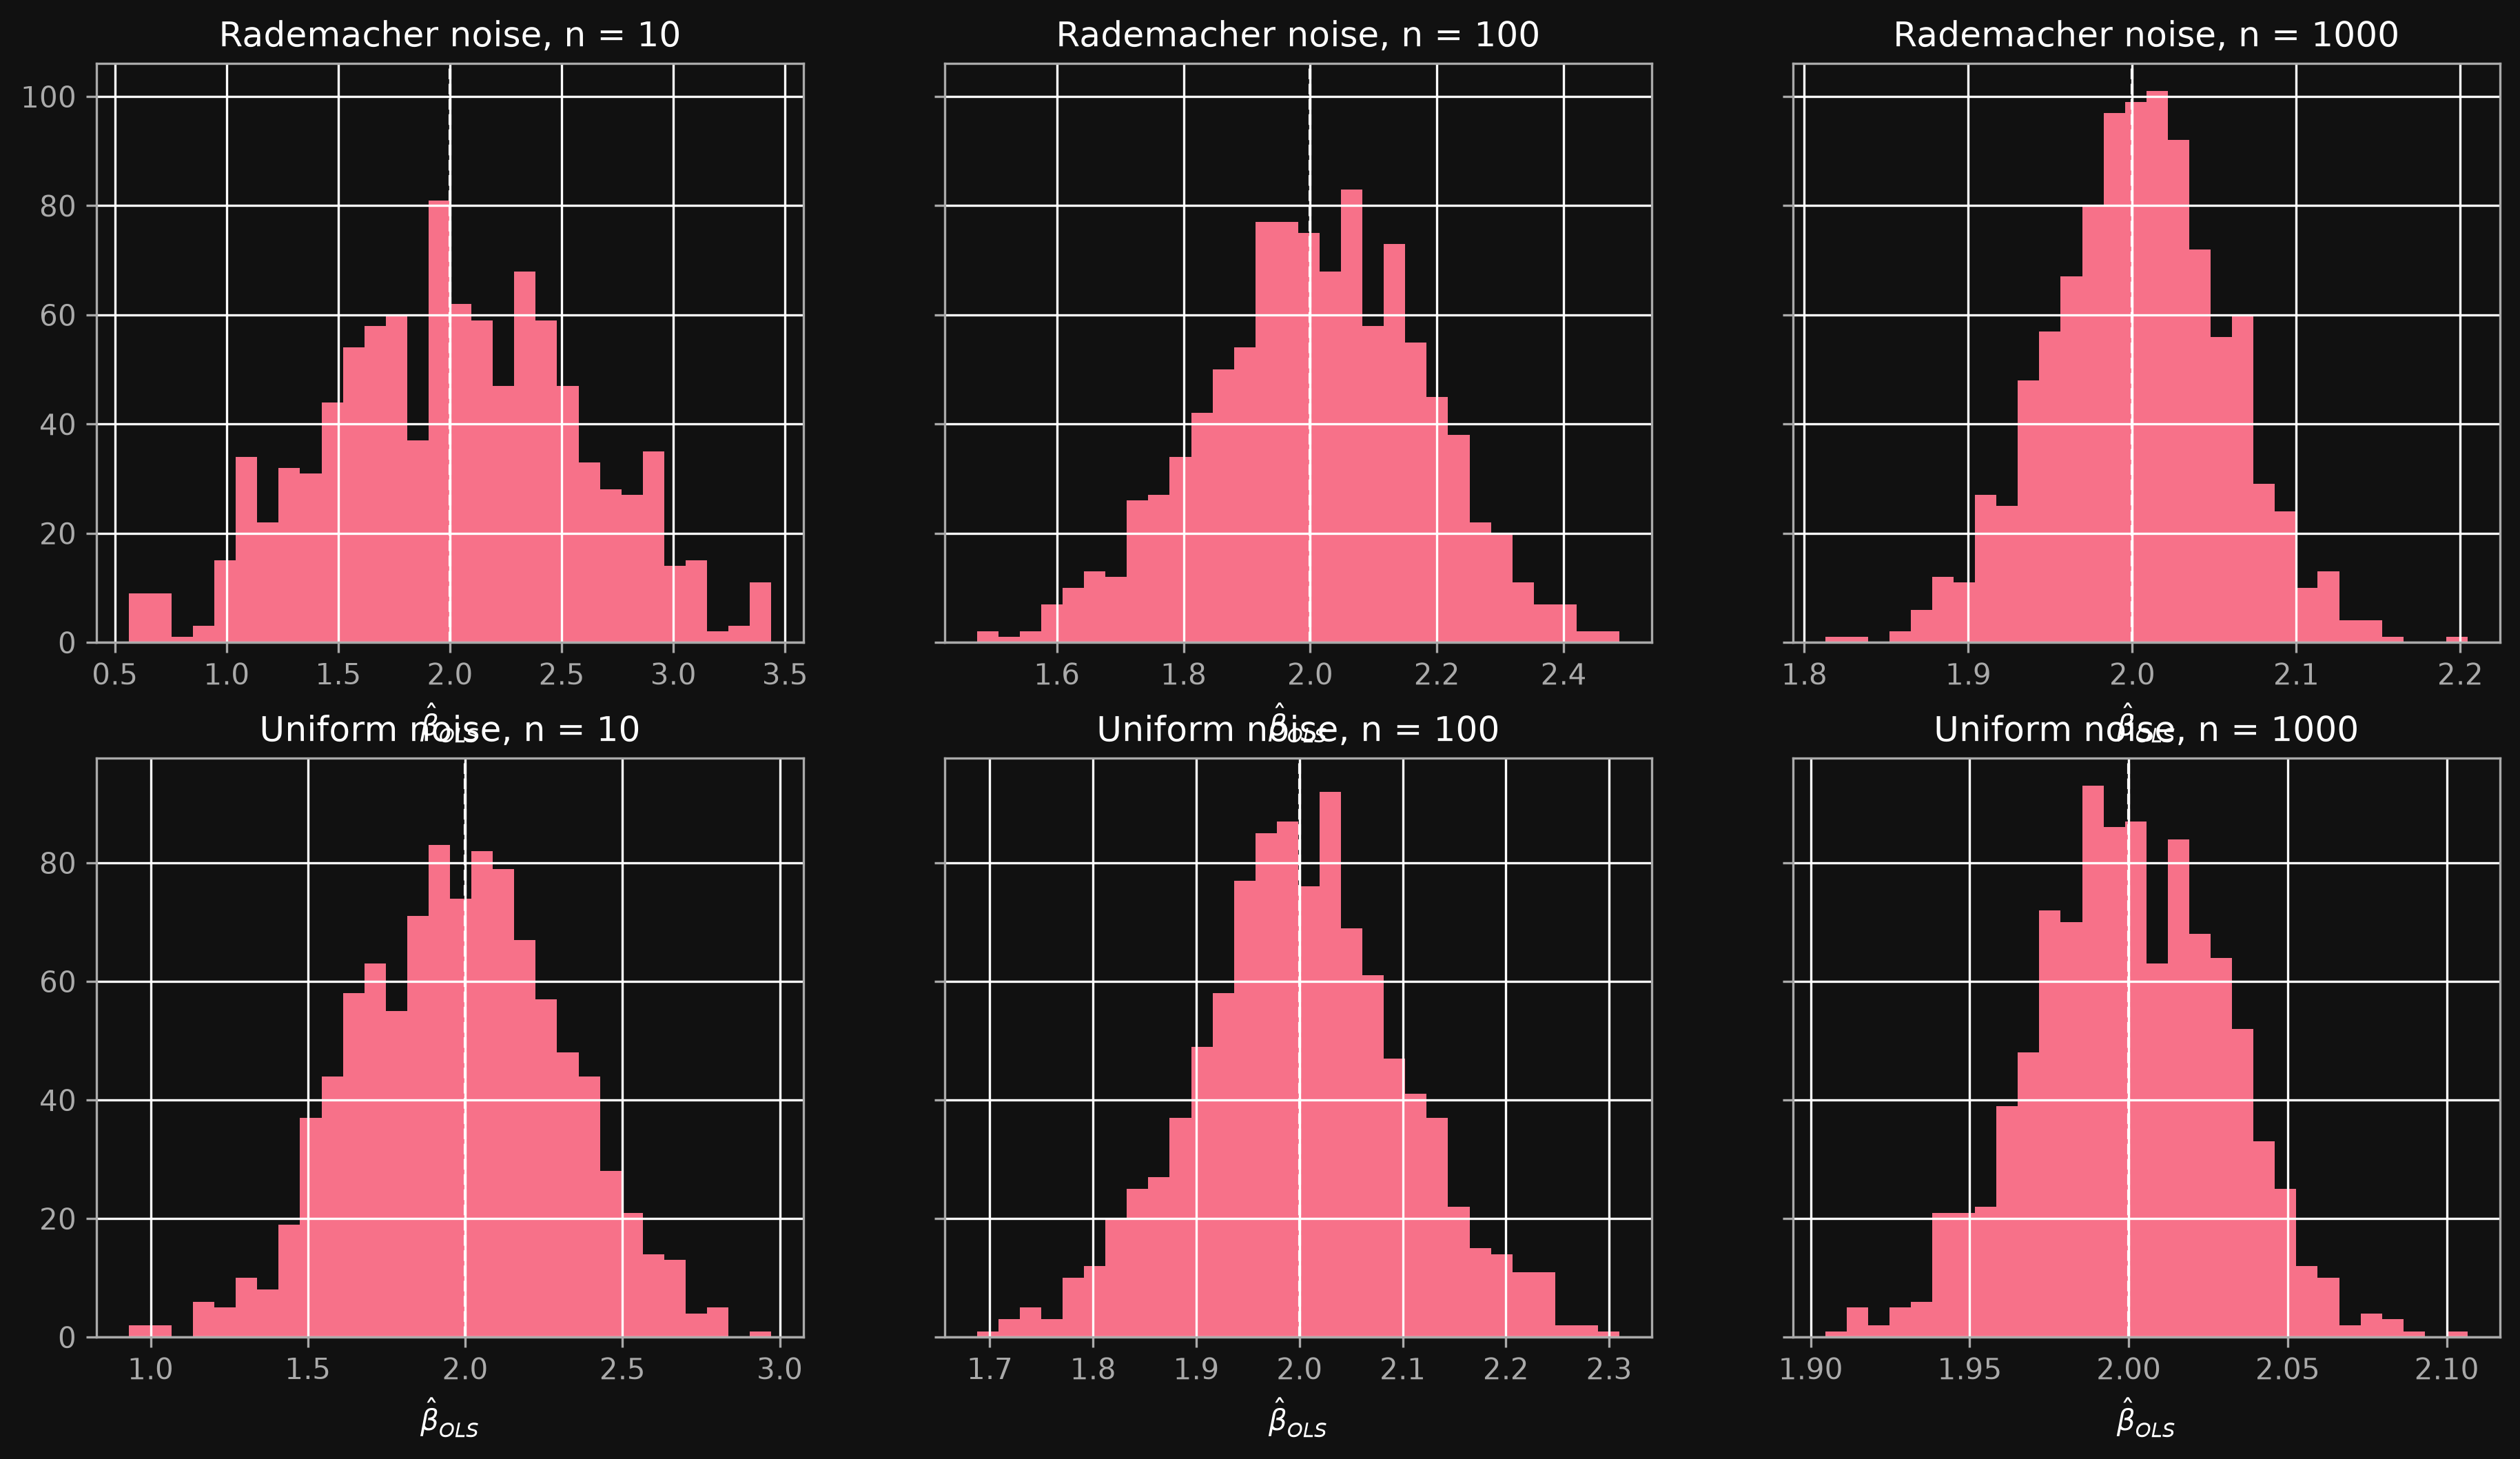
\includegraphics[width=0.68\textwidth]{./figures/problem2_beta_histograms.png}
\end{center}

\begin{center}
\begin{tabular}{lrrrrrr}
\toprule
 & 10\_beta1 & 10\_beta2 & 100\_beta1 & 100\_beta2 & 1000\_beta1 & 1000\_beta2 \\
\midrule
shapiro\_stat & 0.9953 & 0.9983 & 0.9976 & 0.9983 & 0.9991 & 0.9988 \\
shapiro\_p & \textbf{0.0038} & 0.4183 & 0.1475 & 0.4453 & 0.9025 & 0.7548 \\
\bottomrule
\end{tabular}
\end{center}

(\texttt{beta1} is the Rademacher noise, \texttt{beta2} the uniform.)

Only one cell rejects normality: Rademacher noise at $n = 10$, with $p = 0.0038$. Its p-value then
climbs to $0.1475$ at $n = 100$ and $0.9025$ at $n = 1000$, which is the central limit theorem doing
its work on a noise term that is not remotely normal.

The uniform noise never rejects, not even at $n = 10$. An average of ten uniforms is already close
to normal, whereas ten two-point draws are not, so the two distributions need different sample sizes
before the same conclusion holds.


\problem{3: Weighted Least Squares}

This problem focuses on verifying the findings of Class 2 regarding
Weighted Least Squares (WLS).

\subproblem{3.1: Setup}

Similar to before, define the true model as:
$$
y = 2x
$$
Where $x$ is sampled from the uniform distribution $x \sim \text{Uniform}(1, 2)$.

Second, define the noise $\epsilon_i$ to be sampled from a normal distribution with mean 0,
and variance $\sigma_i^2$ that depends on $x_i$ as follows:
$$
\sigma_i^2 = \frac{1}{x_i^2}
$$

For $n=500$, please plot the generated data points $(x_i, y_i + \epsilon_i)$.

\answer
The true model has no intercept, so every fit below is through the origin, and the noise enters the
response: $y_i = 2 x_i + \epsilon_i$ with $\epsilon_i \sim \mathcal{N}(0,\, 1/x_i^2)$. That is what
makes $w_i = x_i^2$ the correct weights in 3.5, since $w_i = 1/\sigma_i^2$.

\begin{lstlisting}[language=Python]
np.random.seed(3)

n = 500
x = np.random.uniform(1, 2, n)
sigma = 1 / x
eps = np.random.normal(0, sigma)
y = 2 * x + eps
\end{lstlisting}

\begin{center}

\includegraphics[width=0.68\textwidth]{./figures/problem3_scatter.png}
\end{center}

The vertical spread is widest at $x = 1$ ($\sigma_i = 1$) and narrowest at $x = 2$
($\sigma_i = 1/2$), which is the heteroskedasticity we built in.


\subproblem{3.2: Naive OLS}

Fit a standard OLS regression to the data generated above.

Report your estimate $\hat{\beta}_{\text{OLS}}$, and the confidence interval for the estimate.

\answer
\begin{center}
\begin{tabular}{lcccccc}
\toprule
            & \textbf{coef} & \textbf{std err} & \textbf{t} & \textbf{P$> |$t$|$} & \textbf{[0.025} & \textbf{0.975]}  \\
\midrule
\textbf{x}  &       2.0087  &        0.021     &    97.590  &         0.000        &        1.968    &        2.049     \\
\bottomrule
\end{tabular}
\end{center}

$\hat{\beta}_{\text{OLS}} = 2.0087$, with a 95\% interval of $[1.9683,\, 2.0491]$. The point estimate
is fine -- OLS is still unbiased under heteroskedasticity. What is wrong is the standard error.


\subproblem{3.3: Interpretation}

Briefly discuss whether naive OLS will be under or over confident in its estimate of $\hat{\beta}_{\text{OLS}}$,
and why.

\answer
\textbf{Under-confident}: the reported interval is wider than it needs to be.

For a fit through the origin, $\hat{\beta} - \beta = \sum_i x_i \epsilon_i / \sum_i x_i^2$, so the
true variance is
$$
\Var(\hat{\beta}_{\text{OLS}}) = \frac{\sum_i x_i^2 \sigma_i^2}{\left(\sum_i x_i^2\right)^2}
= \frac{\sum_i x_i^2 \cdot (1/x_i^2)}{\left(\sum_i x_i^2\right)^2}
= \frac{n}{\left(\sum_i x_i^2\right)^2},
$$
whereas OLS \textit{reports} $\bar{\sigma}^2 / \sum_i x_i^2$, charging every point one common
variance. The ratio of reported to true variance is
$$
\frac{\bar{\sigma}^2 \sum_i x_i^2}{n} \;\longrightarrow\;
\E\!\left[\tfrac{1}{x^2}\right] \E\!\left[x^2\right] = \frac{1}{2} \cdot \frac{7}{3} = \frac{7}{6},
$$
so the reported standard error is about $\sqrt{7/6} \approx 1.08$ times too large.

In a fit through the origin the large-$x$ points carry the most weight, and those are exactly the
points with the \textit{smallest} noise, since $\sigma_i = 1/x_i$. OLS charges them the average
noise level instead, so it overstates its own uncertainty. The heteroskedasticity-robust (HC3)
standard errors confirm it:

\begin{center}
\begin{tabular}{lrrrr}
\toprule
 & $\hat{\beta}$ & std err & CI lower & CI upper \\
\midrule
OLS (conventional) & 2.00870 & 0.02058 & 1.96826 & 2.04914 \\
OLS (HC3 robust)   & 2.00870 & 0.01908 & 1.97131 & 2.04610 \\
\bottomrule
\end{tabular}
\end{center}

The realized ratio of the two standard errors is $1.0788$, against the $1.0801$ the algebra
predicts in the limit.

Note that the direction is specific to this design. If the variance \textit{grew} with $x$ instead,
the heavily weighted points would be the noisy ones and naive OLS would be over-confident.


\subproblem{3.4: Visualization}

Plot a Q-Q plot of the residuals from the naive OLS regression. What do you observe?

\answer
\begin{center}
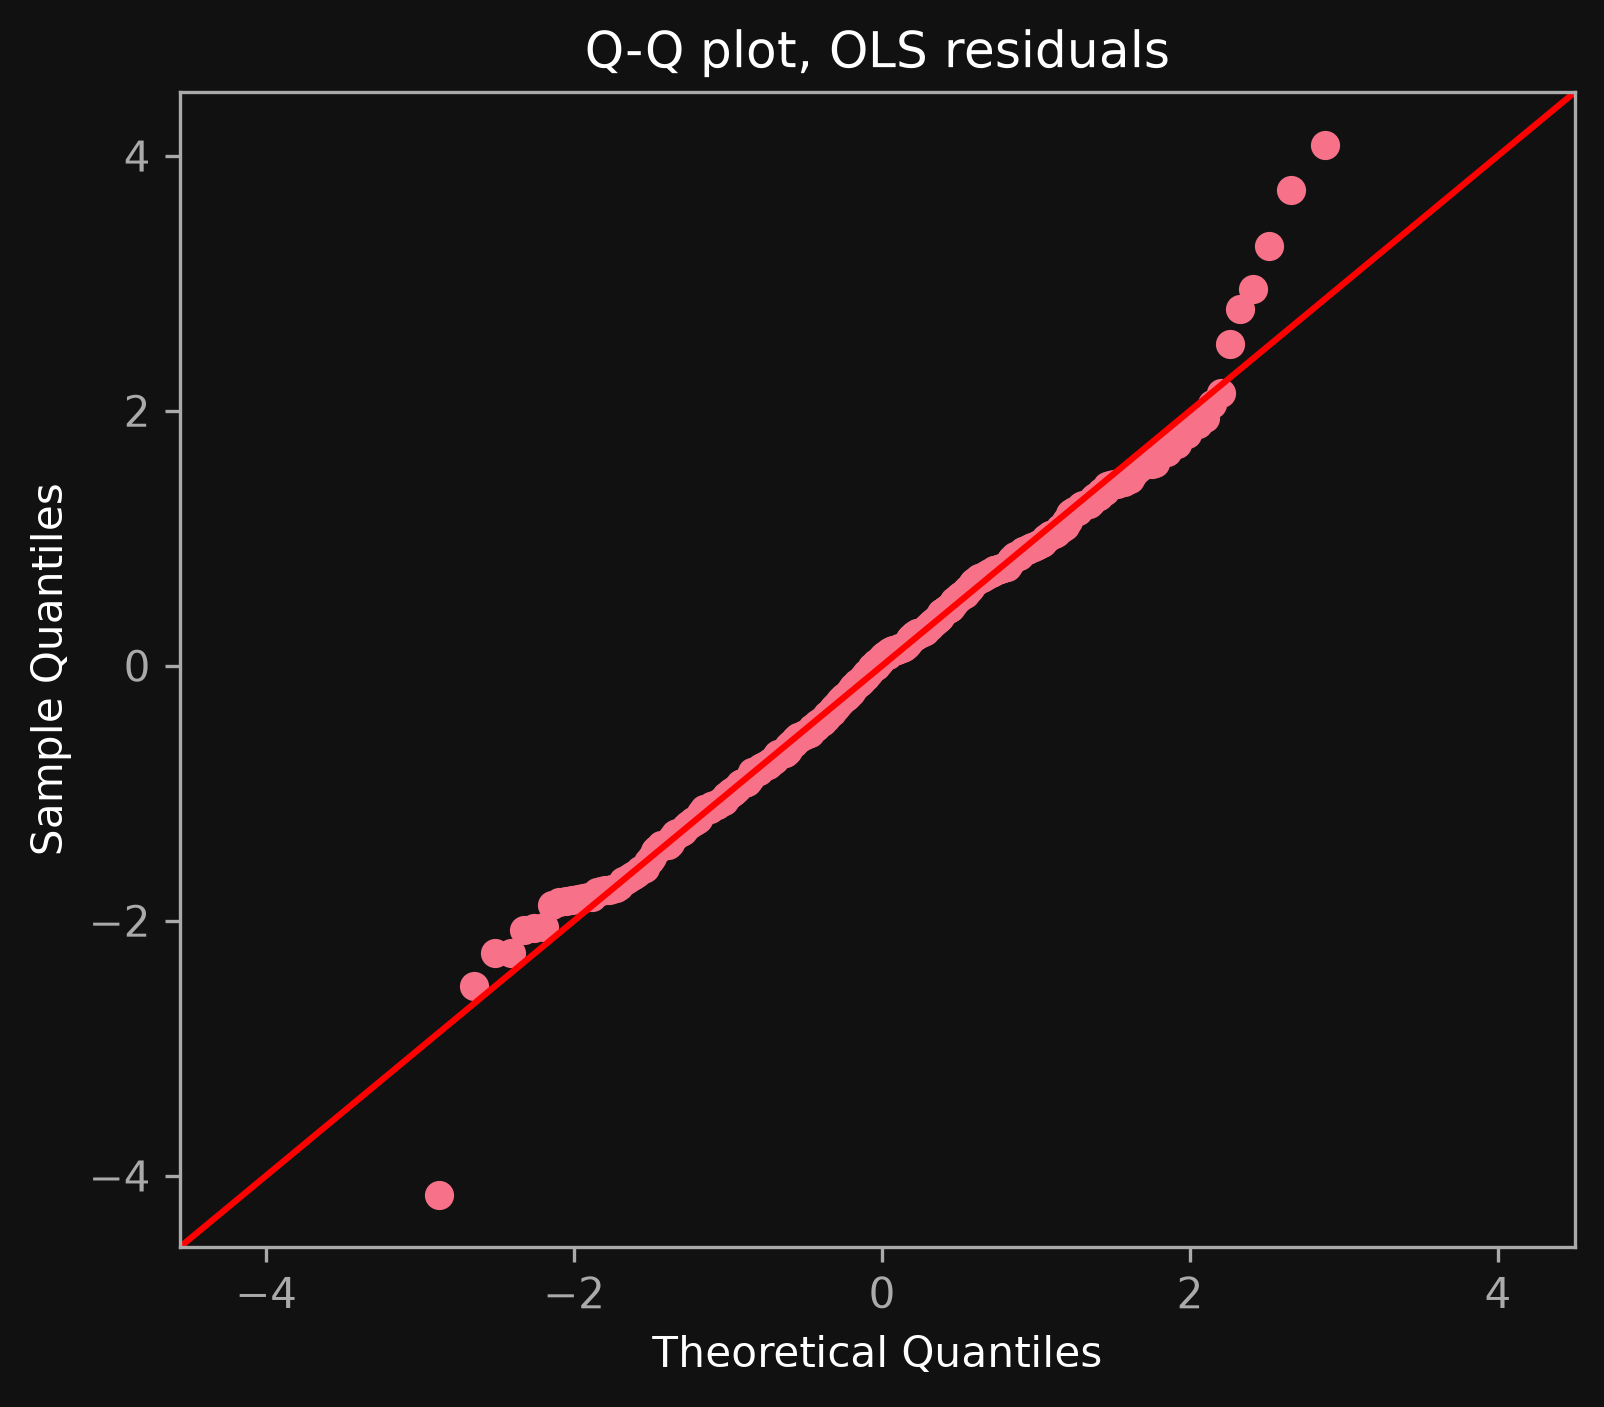
\includegraphics[width=0.58\textwidth]{./figures/problem3_OLS_qq_plot.png}
\end{center}

The points bend away from the $45^\circ$ line in both tails. Each $\epsilon_i$ is normal on its own,
but the residuals pool draws from 500 \textit{different} variances -- a scale mixture of normals,
which is not itself normal. Shapiro-Wilk gives $p = 0.0011$.


\subproblem{3.5: Weighted Least Squares}

Fit a Weighted Least Squares regression to the data generated above, using weights $w_i = x_i^2$.
Report your estimate $\hat{\beta}_{\text{WLS}}$, and the confidence interval for the estimate.

\answer
\begin{center}
\begin{tabular}{lcccccc}
\toprule
            & \textbf{coef} & \textbf{std err} & \textbf{t} & \textbf{P$> |$t$|$} & \textbf{[0.025} & \textbf{0.975]}  \\
\midrule
\textbf{x}  &       2.0113  &        0.018     &   112.329  &         0.000        &        1.976    &        2.046     \\
\bottomrule
\end{tabular}
\end{center}

$\hat{\beta}_{\text{WLS}} = 2.0113$, with a 95\% interval of $[1.976,\, 2.046]$. The weights
$w_i = x_i^2 = 1/\sigma_i^2$ are exactly the GLS weights, so this is the efficient estimator: its
standard error of $0.018$ beats both the conventional and the robust OLS numbers from 3.3.


\subproblem{3.6: Visualization}

Plot a Q-Q plot of the weighted residuals from the WLS regression. What do you observe compared
to the Q-Q plot from the naive OLS regression?

\answer
\begin{center}
\begin{minipage}{0.48\textwidth}
    \centering
    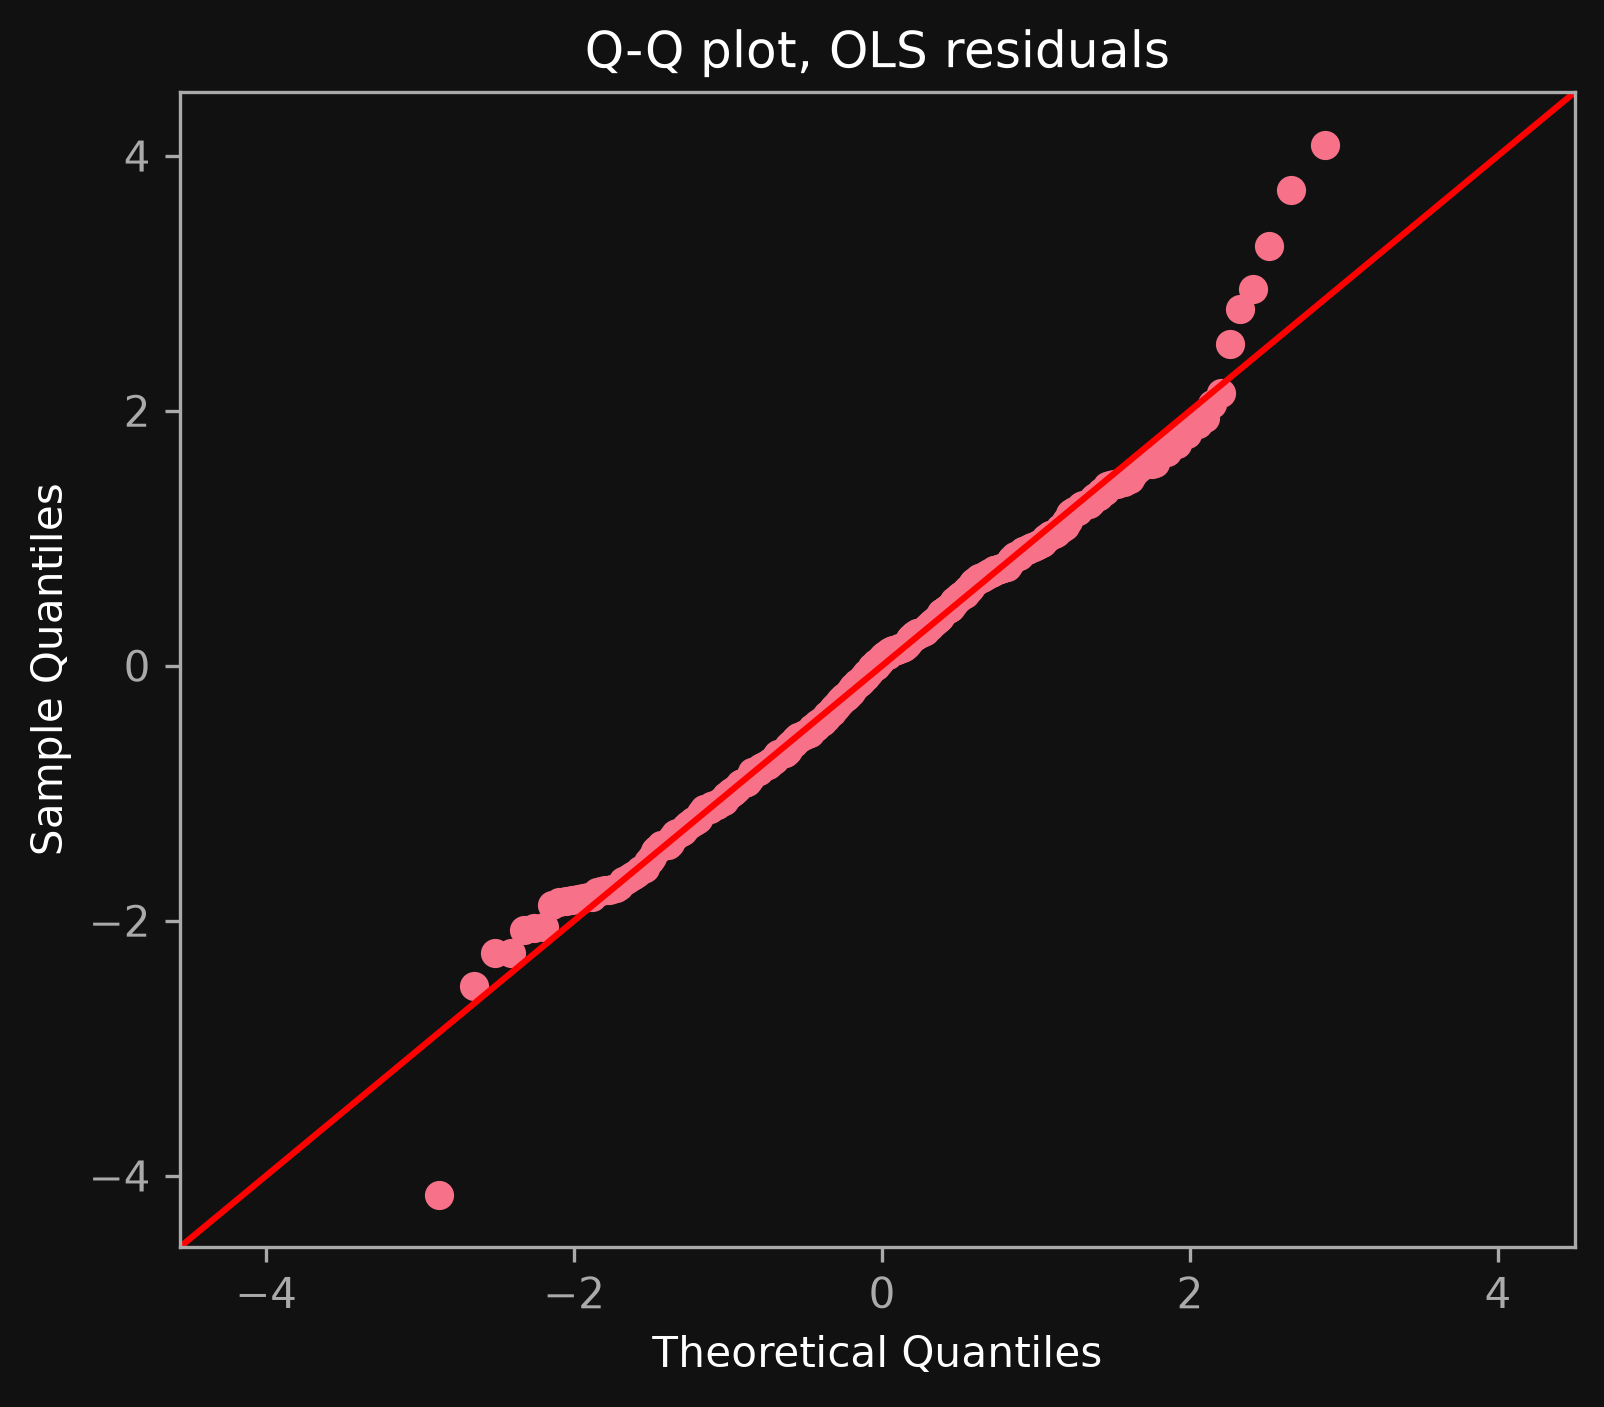
\includegraphics[width=\textwidth]{./figures/problem3_OLS_qq_plot.png}\\[3pt]
    Naive OLS
\end{minipage}
\hfill
\begin{minipage}{0.48\textwidth}
    \centering
    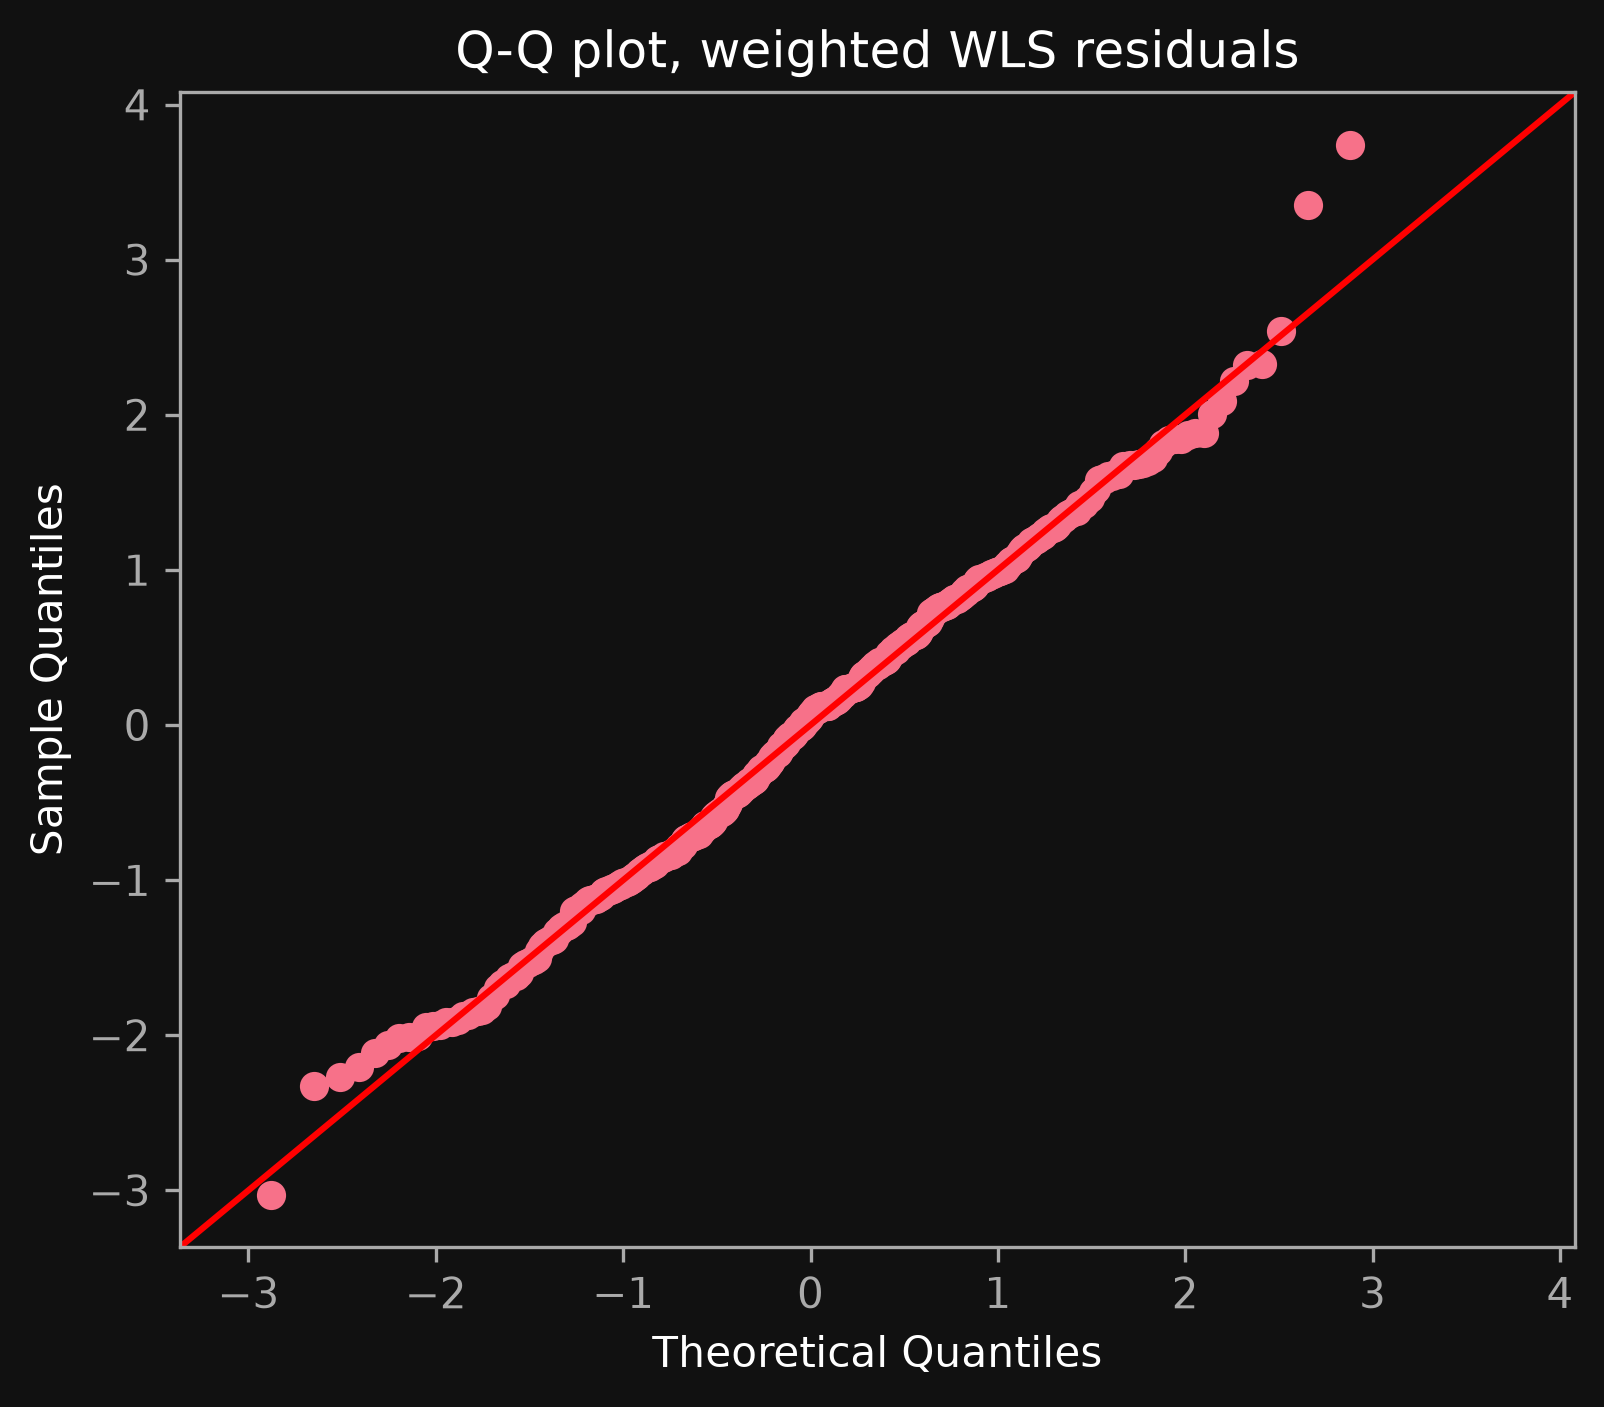
\includegraphics[width=\textwidth]{./figures/problem3_WLS_qq_plot.png}\\[3pt]
    WLS, weighted residuals
\end{minipage}
\end{center}

Much straighter, and the reason is exact: the weighted residual is
$\sqrt{w_i}\, \epsilon_i = x_i \epsilon_i$, which has variance $x_i^2 \cdot (1/x_i^2) = 1$ for
\textit{every} $i$. Weighting turns the scale mixture back into a single standard normal.

\begin{center}
\begin{tabular}{lrrr}
\toprule
 & std dev & Shapiro $p$ & corr($|\hat{\epsilon}|$, $x$) \\
\midrule
OLS residuals            & 0.6994 & 0.0011 & -0.2577 \\
Weighted (WLS) residuals & 0.9852 & 0.1190 & -0.0024 \\
\bottomrule
\end{tabular}
\end{center}

Note that \texttt{model\_wls.resid} returns the \textit{raw} residuals $y_i - x_i \hat{\beta}$, which
are still heteroskedastic. The weighted ones are \texttt{model\_wls.wresid}.


\end{document}
